%!TEX root = TQFTbook.tex
%%%%%%%%%%%%%%
\chapter{2d TQFT with defects}\label{c:2d-defects}


So far we only considered TQFTs defined on homogeneous spacetimes, where the
local structure of the theory is the same at every point of the spacetime.
However, one can also consider theories where different parts of the spacetime
carry different TQFTs. The codimension-one locus separating the homogeneous
parts should describe interface between different TQFTs; moreover, one can
continue, introducing a codimension 2 stratum separating different codimension
1 interfaces. In physics, all these positive codimension strata are thought of
as a \emph{defects}\index{defect} in the structure of spacetime, and the
corresponding formalism is referred to as \emph{TQFT with
defects}\index{TQFT!with defects}. As we will show later, this approach
is very closely related to fully extended TQFT (see section FIXME below).

This idea has a long history in physics. Our exposition follows  \cite{dkr},
which gives a detailed description of 2D TQFT with defects. See also review
articles \cite{carqueville} and \cite{cdr}. Very closely related formalism in
the context of extended TQFTs is also described in \cite[Section 4.3]{lurie}
under the name \emph{TQFT for manifolds with singularity}. For simplicity, we
restrict ourselves to the 2-dimensional case.

% Wrapping the Tikz commands in an environment so that they don't interefere with other chapters.
\begin{defectfiguresetup}
%%%%%%%%%%%%%%%%%%%%%%%%%%%%%%%%%%%%%%%%%%%%%%%%%%%%%%%%%%%%%
\section{Data for TQFT with defects}\label{s:defect-data}
Recall that we have defined a two-dimensional extended TQFT as a symmetric
monoidal functor $Z\colon \Bord_2\to \calC$, where $\calC$ is a (weak)
2-category; such a theory is uniquely determined by a fully dualizable object
$A\in \calC$. In particular, it assigns an invariant $Z_A(M)\in
\End_\calC(\one)$ to every closed manifold $M$; equivalently, we can say that
it assigns an invariant $Z(M,A)$ to every pair $(M, A)$, where $M$ is a closed
2-manifold and $A\in \calC$ is a fully dualizable object. We can think of pair
$(M,A)$ as a \emph{colored manifold}, i.e. a manifold together with some extra
data (coloring), which in this case consists of choosing an object $A$.

For theory with defects, we need to modify this definition in two ways. First,
instead of usual bordisms, we need to define bordisms with defects,  as
outlined in introduction to this chapter. Second, we neeed to define the notion
of coloring, i.e. assignign appropriate alegbraic data to different strata.
Aftre that, we will be able to define an extended TQFY with defects as a
symmetric monoidal functor
$$
Z^{\mathrm{defect}}\colon \Bord_2(\calC)\to \calC.
$$
where $\Bord_2(\calC)$ is the 2-category of $\calC$-colored stratified oriented
2-bordisms.


We begin by defining closed manifolds
with defects, or \emph{stratified manifolds}.

\begin{definition}\label{d:stratified_manifold}
  A \emph{stratified 2-manifold}\index{stratified manifold} is an
  oriented closed 2-manifold $M$ together with  decomposition
  $$
    M=M_2\sqcup M_1\sqcup M_0
  $$
  where each $M_i$ is a (not necessarily compact) locally closed submanifold
  of dimension $i$ in $M$ such that:
  \begin{itemize}
    \item $M_2$ is open and dense in $M$
    \item Every point $x\in M_1$ has a neighborhood which looks like shown in
    FIXME
    \item Every point $x\in M_0$ has a neighborhood which looks like shown in
    FIXME
  \end{itemize}
\end{definition}
We will refer to $M_1$ and $M_0$ as strata of dimension 1 (respectively, 0);
physicists would also call them defect lines and point defects respectively.

An example of a stratified manifold is shown in
\firef{f:stratified_pretzel} below.

In a similar way one can define the notion of a stratifed manifold with boundary
or a stratified cobordism; in this case, we need to require additionally that
the stratification meets the boundary transversally (in particular, it means
that the codimesion 2 strata should not be on the boundary).


	\begin{figure}[ht]
	\centering
	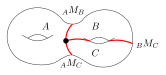
\includegraphics{figures/c13-fig01.svg}
	\caption{A stratified manifold decorated with algebras $A$, $B$ and $C$ on
	different regions. Defects are shown in red, and are labelled by bimodules.
	Defects require a choice of orientation, which is suppressed here for
	brevity.}
	\label{f:stratified_pretzel}
\end{figure}

Next, we should define the notion of coloring. We do it first in a very special
case, namely when the manifodl $M$ is closed and the target category $\calC$ is
the category of associative algebras. As was previously discussed, fully
dualizable objects in this category are finite-dimensional semisimple algebras,
and for construction of an extended TQFT one needs a semisimple algebra with
extra data, namely with the structure of a symmetric Frobenius algebra.

Before the continuing, let us note that we assume that $M$ is oriented;
however, we do not assume any choice of orientation on defect lines (that is,
connected components of $M_1$). Note that since $M$ is oriented, choosing an
orientation of $M_1$ is equivalent to chooisng orientation of the normal bundle
to $M_1$

\begin{definition}\label{d:defect-coloring}
  Let $M$ be a closed oriented stratified 2-manifold, and let $\calC=\Alg$ be
  the 2-category of alegbras and bimodules as defined in \exref{x:alg}. A
  $\calC$-coloring of $M$ is the following data:
  \begin{itemize}
    \item A choice of a semisimple symmetric Frobeinus algebra $C(U)$ for each
    connected component $U$ of the open strata $M_2$

    \item A choice of a 1-morphism (that is, a bimodule) $M=C(Y)$ for every
    connected component $Y$ of $M$ together with orientation of $Y$. More
    precisely, if $Y$ separates regions colored by algebras $A$ and $B$ as
    shown below, then it should be colored by a finite-dimensional  $B$-$A$
    bimodule $M$.

    Moreover, we require that the bimodules corresponding to opposite choice of
    orientation are duals (in the sense of vectro spaces) of each other. FIXME:
    better wording.

    \item
        For each vertex $u \in M_0$, we need a multilinear map $\ph_u$ from
        cyclic tensor product of incident bimodules to the field $\kk$.

    		\begin{figure}[ht]
    			\centering
    			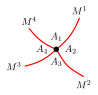
\includegraphics{figures/c13-fig02.svg}
    			\label{f:junction}
    		\end{figure}

    		For example, if the junction looks like as given above, then it is
    		assigned a map:

    		\begin{equation}\label{e:junction-data}
    			\varphi: \circlearrowleft_{A_1} ( M^1 \otimes_{A_2}  M^2
    			\otimes_{A_3} M^3 \otimes_{A_4} M^4  ) \rightarrow  \kk
    		\end{equation}

    		 Here, $\circlearrowleft_{A} M$ is the cokernel of the map $A \otimes M
    		 \rightarrow M, a \otimes m \mapsto am - ma$. This property of
    		 $\varphi$ ensures that the junction has no preferred starting edge.
    		 See \cite[Section 2.3]{carqueville} for another motivation behind
    		 this data.
  \end{itemize}
  We will refer to a pair $(M, C)$, where $M$ is an oriented manifold and $C$
  is $\calC$-coloirng of $M$ as a \emph{$\calC$-colored
  manifold}.\index{stratified manifold!$\calC$-colored}
\end{definition}

%%%%%%%%%%%%%%%%%%%%%%%%%%%%%%%%%%%%%%%%%%%%%%%%%%%%%
\section{State sum construction of TQFT with defects}\label{s:defect-statesum}

In this section we sketch the construction of the TQFT with defects, i.e., a
functor $Z^{\mathrm{defect}}\colon \Bord_2(\calC)\to \calC$, using state sum
approach.  As before, we only consider the target category $\calC=\Alg$. For
simplicity, in this section we only explain how one defines $Z(M,C)$ for a
colored stratified closed 2-manifold $M$; generalization of this to cobordisms
will be explained in the next section. Our exposition follows \cite{dkr} with
minor changes, though their notation differs from ours (in particular, they use
$T^{\mathrm{cw}}$ for what we denote by $Z\equiv Z^{\mathrm{defect}}$).

The state sum construction below is a generalization of construction in
\chref{c:2d-lattice}. Thus, given $\calC$-colored stratified closed 2-manifold
$M$, we begin by choosing a PLCW decomposition $K$ of it; we require that this
PLCW decomposition is transversal to the stratification.


As in \seref{s:state-sum}, we denote by $K_2$ the set of 2-cells of $K$, by
$K_1$ the set of 1-cells (edges), and by  $K_0$, the set of vertices. Further,
we assume that every edge $r\in K_1$ has at most one intersection with the
defect lines, i.e. stratum $M_1$, and each 2-cell $F$ of the decopmosition
contains at most one point from $M_0$. An examples of such PLCW decomposition
of a stratified manifold is shown in \firef{f:vectors-on-edges}.



As in \seref{s:state-sum}, we will denote by $E$ the set of \emph{oriented}
edges of $K$, i.e., pairs consisting of an edge $r\in K_1$ and an orientation
of $r$. Thus, every (unoriented) edge $r\in K_1$ gives rise to two oriented
edges $r', r''\in E$. To every oriented edge $r\in E$, we assign a vector space
$Q_r$ s follows:
\begin{equation}\label{e:q-definition}
	Q_{r} =
	\begin{cases}
		A, & \text{if $r$ does not cross a defect line and lies within component of
		$M_2$ colored by algebra $A$ },\\
		X, & \text{if $r$ crosses defect line which is colored by bimodule $X$,
    with orientation as shown below FIXME}
	\end{cases}
	\end{equation}

We define an intermediate vector space $Q(M)$ by tensoring the contribution of
\begin{equation}\label{e:Qr}
	Q(M) = \bigotimes_{r\in E} Q_r.
\end{equation}
Note that in the special case of a manifold without stratification, this
coincides with vector space $A^E$ as defined in \eqref{e:AE}.

Note that each (unoriented) edge $r\in K_1$ gives two factors in $Q(M)$: either
two copies of $A$ (if $r$ does not intersect defect lines) or $X\otimes X^*$,
where $X, X^*$ are the colors of of the defect line crossing $r$ (one
orientation gives $X$, the other, $X^*$).


FIXME

Consider  \firef{f:vectors-on-edges} for example. Edge $e_2$, irrespective of
its orientation, lies entirely in algebra $b$, so it is labelled $A_b$. Edge
$e_1$, within polygon $p_2$, has defect $x$ crossing it such that the defect is
entering $p_2$.  So the triplet $(p_2,e_1,+)$ is labelled $X_x$. The same edge,
within polygon $p_1$, has defect $x$ going out of the polygon. So it is
labelled $X_x^*$ for the triplet $(p_1,e_1,+)$.  We only consider those
triplets where the orientation matches with that of the polygon. We would have
to consider both orientations of an edge ( i.e. for example $(p_1,e_1,+)$ as
well as $(p_1,e_1,-)$ ) only when the polygon closes on itself through that
edge. See \cite[Section 3.5]{dkr} for an example.

\begin{figure}[ht]
	\centering
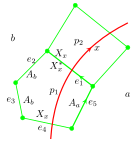
\includegraphics{figures/c13-fig03.svg}
			\caption{Example of vector spaces assigned to the edges of 2-cell $p_1$. Regions to the left and right of defect $x$ are labelled by algebras $b$ and $a$ respectively.}
			\label{f:vectors-on-edges}
\end{figure}

Next, for every (unoriented) edge $r$ we define a vector
$$
e_r = \sum x_i \otimes x^i\in Q_{r'}\otimes Q_{r''}
$$
where $r'$, $r''$ are two orientations of $r$. Namely,
\begin{itemize}
  \item If $r$ doesn't intersect defect lines so that $Q_{r'}\otimes
  Q_{r''}=A\otimes A$, then $x_i, x^i$ are dual bases in $A$ with respect to
  Frobenius pairing (compare with \eqref{e:er}).
  \item If $r$ intersects a defect line labelled by bimodule $X$ or $X^*$
  (depending on orientation), then $x_i, x^i$ are dual bases in $X$, $X^*$.
\end{itemize}

Taking product over all unoriented edges $r\in K_1$, we get a vector
$$
e_M=\bigotimes_{r\in K_1} e_r\in Q(M)
$$
(compare with \eqref{e:eM}).


FIXME: algebraic data defined by vertices??


Finally, for a 2-cell $F$ of $K$, we define the space
$$
Q_F=\bigotimes_{r\in \ov{\del F}}Q_r
$$
where the tensor product is taken in clockwise order, and
a map
$$
\eps_F \colon Q_F\to \kk
$$
as follows.

\begin{enumerate}
	\item[I.]
    If the 2-cell contains a single vertex $v\in M_0$, and for each edge $r$ of
    $F$ there is a unique defect line passing through that edge, then we
    define
    \begin{equation}
      \eps_F=\ph_v\colon X_1\otimes_{A}\dots \otimes X_k\to \kk
		\end{equation}
    (the product is taken in clockwise order).

    If $F$ contains a vertex, but certain edges don't intersect any defect
    lines, we multiply the colors of these edges and the color of the adjacent
    bimodule elements, as illustrated by the figure below.

FIXME

  \item[II.]
    If the cell $F$ has no vertex and contains a unique defect line, colored by
    $X$ and crossing two edges of $F$, then we add on this line a single vertex
    $v$ colored by $\ph_v=\ev_X\colon X^*\otimes X\to \kk$, and then use the
    previous construction.

	\item[III.] If no defect line passes through $F$, and $F$ lies in region
    labelled by algebra $A$, then
    $$
    \eps_F(a_1 \otimes \cdots\otimes  a_k) = \eps_{A}(a_1 \cdots a_k)
    $$
    (compare with \eqref{e:epsF}).
\end{enumerate}

Note that case  III can be considered as special case of I, if we allow
ourselves adding ``trivial'' defect lines, colored by ${}_AA_A$,  in any region
colored by algebra $A$.

As before, taking the tensor product over all 2-cells  $F\in K_2$ and observing
that $\bigotimes_F Q_F=Q(M)$ (which follows from the fact that every unoriented
edge of $K$ appears exactly twice as a boundary of some 2-cell, with opposite
orientations), we can define the map
$$
\eps_M=\bigotimes_{F\in K_2} \eps_F \colon Q(M)\to \kk.
$$

We now define the invariant of a $\calC$-colored stratified manifold $M$
with a given cell decomposition $K$ by
\begin{equation}\label{e:defect-state-sum}
  Z(M,C,K)=\eps_M (e_M)
\end{equation}
(compare with \eqref{e:fhk-state-sum}). FIXME: $w^{-1}$??


The functor $Z$ for a bordism $M:U\rightarrow V$ is defined as:
\begin{equation}
	Z(M) : Z(U) \xto{id_{Z(U)} \otimes P(M)} Z(U) \otimes Q(M) \otimes Z(V) \xto{E(M) \otimes id_{Z(V)}} Z(V)
\end{equation}

We explain $Z(U), Z(V), P(M), E(M)$ next.


Let's define the functor on a (decorated) circle $O$ first. For a more general object $U=O_1 \sqcup O_2 \sqcup \cdots \sqcup O_n$, we then have $Z(U)=Z(O_1)\otimes Z(O_2) \otimes \cdots \otimes Z(O_n)$. As a 1-dimensional space, a circle doesn't need 2-cells for its decomposition.  \cite[Section 2.3]{dkr} provides a construction using collars to assign a vector space to decorated circles with just this data. But we will reuse the following equivalent boundary convention. For a circle $O$ lying on $\partial_{in} M$, we assign the same vector space to each edge as was defined in \eqref{e:q-definition}. For a circle lying on $\partial_{out} M$, we still use the \eqref{e:q-definition}, but dualize the $X$ type vector spaces.

The map $P(M): \kk \rightarrow Q(M) \otimes Z(V)$ is defined as:
\begin{equation}
	P(M) = \bigotimes_{e \in C_1(M), e \notin \partial_{\mathrm{in}} M} P_e
\end{equation}

For an edge $e$ intersecting a defect $x$, the propagator map $P_e: \kk \rightarrow Q_{p(e)_1,e,\mathrm{or}_1} \otimes Q_{p(e)_2,e,\mathrm{or}_2}$ comes from a basis $\sum_{i} u_i \otimes u_i^* \in X_x \otimes X_x^*$. For an edge that does not intersect any defect, and is contained in Frobenius algebra $a$, the map $P_e$ comes from the coevaluation map $\beta_{A_a}$ of the algebra $a$.

We then define the evaluation map $E_p: \bigotimes_{(e,\mathrm{or}) \in \partial p} Q_{p,e,\mathrm{or}} \rightarrow \kk $ for each polygon $p$ as:
\begin{enumerate}
	\item[I.] If no defect line passes through $p$, and $p$ lies in region labelled by algebra $a$, then $E_p(q_1 \otimes \cdots q_m) = \eps_{A_a}(q_1 \cdots q_m)$. This is the same map which was used for TQFT without defects ( see  \eqref{e:k-pairing} ).
	\item[II.] Let's say a defect line $x$  passes through two edges such that $q_1 \in X_x^*$ ( outgoing ) and $q_i \in X_x$ ( incoming) , then $E_p(q_1 \otimes \cdots q_m) = q_1 ( (q_2 \cdots q_{i-1}).q_i.(q_{i+1}\cdots q_m))$. Recall that $q_i$ is a bimodule on which appropriate algebra elements can act from right or left sides, and $q_1$ lives in the dual bimodule space.
	\item[III.] If the 2-cell contains a junction such that one domain wall passes through each edge of the 2-cell, we use the map $\varphi_p$, defined in \eqref{e:junction-data}, to assign an element of $\kk$ as:
	\begin{equation}
		E_p(q_1 \otimes \cdots \otimes q_m)=\varphi_p \circ \pi_\otimes(q_1 \otimes \cdots \otimes q_m)
	\end{equation}
	$\pi_\otimes: X_{x_1}^{\epsilon_1} \otimes_{A_2} \cdots \otimes_{A_m}  X_{x_m}^{\epsilon_m} \rightarrow \circlearrowleft_{A_1} (X_{x_1}^{\epsilon_1} \otimes_{A_2} \cdots \otimes_{A_m}  X_{x_m}^{\epsilon_m}) $ is a projection to the cylic tensor product on which $\varphi_p$ acts. If $p$ contains a junction, but certain edges don't intersect any domain wall, we can still use this definition of $E_p$ by multiplying its algebra elements with an adjacent bimodule.
\end{enumerate}

%This image is floating into the next section. So I decided to insert it directly instead of inserting as an image
\begin{center}
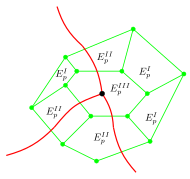
\includegraphics{figures/c13-fig04.svg}
\end{center}

For example, for the defect network shown above, we indicate by subscripts as to which definition of $E_p$ will be used in different polygons. Altogether, the evaluation map $E(M)$ is then defined as:

\begin{equation}
	E(M) = \bigotimes_{p \in C_2(M)} E_p
\end{equation}

This completes the definition of the functor $Z$. In the special case where the bordism has no boundary, we have $\partial_{\mathrm{in}} = \partial_{\mathrm{out}} = \emptyset$. Then $Z$ is just a map from $\kk$ to $\kk$, which is just an element of $\kk$.

\section{Independence of cell decomposition}\label{s:decomposition-independence}
We had to use a cell decomposition in the last section to define the functor $Z$. Since cell decomposition is not a part of the actual defect TQFT data, we need to prove that the state sum construction is independent of our choice of cell decomposition. The key part of the proof is the following lemma.

\begin{lemma}\label{l:invariance-under-local-moves}
	For two colored bordisms $M$ and $M'$, $Z(M) = Z(M')$ if the cell decompositions of $M$ and $M'$ are related by one of the following classes:
	\begin{enumerate}
		\item Addition of an edge with a vertex to a 2-gon

		\newcommand{\twogonA}{%
			\vcenter{\hbox{%
					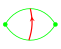
\includegraphics{figures/c13-fig05.svg}%
			}}%
		}

		\newcommand{\twogonB}{%
			\vcenter{\hbox{%
					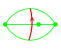
\includegraphics{figures/c13-fig06.svg}%
			}}%
		}

		\newcommand{\twogonC}{%
			\vcenter{\hbox{%
					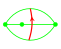
\includegraphics{figures/c13-fig07.svg}%
			}}%
		}

		\begin{align*}
			\twogonA \leftrightarrow \twogonB \leftrightarrow \twogonC
		\end{align*}

		\item Addition of an edge inside an n-gon

		\newcommand{\pentagonA}{%
			\vcenter{\hbox{%
					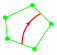
\includegraphics{figures/c13-fig08.svg}%
			}}%
		}

		\newcommand{\pentagonB}{%
			\vcenter{\hbox{%
					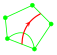
\includegraphics{figures/c13-fig09.svg}%
			}}%
		}

		\newcommand{\pentagonC}{%
			\vcenter{\hbox{%
					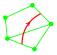
\includegraphics{figures/c13-fig10.svg}%
			}}%
		}

		\newcommand{\pentagonD}{%
			\vcenter{\hbox{%
					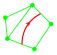
\includegraphics{figures/c13-fig11.svg}%
			}}%
		}


		\newcommand{\pentagonE}{%
			\vcenter{\hbox{%
					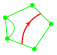
\includegraphics{figures/c13-fig12.svg}%
			}}%
		}

		\begin{align*}
			 \pentagonA \leftrightarrow \pentagonB \leftrightarrow \pentagonC \leftrightarrow \pentagonD \leftrightarrow \pentagonE
		\end{align*}

		Apart from the pentagons shown above, the other diagrams included in this local move are all the n-gons with $n \ge 3$. The domain wall can run between any two edges.
	\end{enumerate}
\end{lemma}

Note that the defect can also be $A$ itself, which is the same as having no defect at all in the diagrams shown above. We sketch here proofs for two of these moves. Let's first consider a move that inserts an edge and a vertex in a 2-gon, as given in \firef{f:example1-local-modification}.

\begin{figure}[ht]
	\centering

	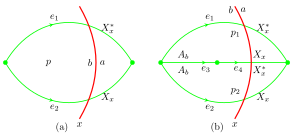
\includegraphics{figures/c13-fig13.svg}

	\caption{Example(I) of a local modification of cell decomposition used in \leref{l:invariance-under-local-moves}}
	\label{f:example1-local-modification}
\end{figure}


The contribution to projector $P$ coming from the new edges $e_3$ and $e_4$ is:
\begin{align*}
	P_{e_3} \otimes P_{e_4}: \kk &\rightarrow (A_b \otimes A_b) \otimes (X_x \otimes X_x^*)\\
												 1 &\mapsto  \sum_i (b_i' \otimes b_i) \otimes \sum_j (u_j \otimes u_j^*)\\
\end{align*}

The total contribution of cells $p_1$ and $p_2$ from the right picture is
\begin{align*}
	& \sum_{i,j} \varphi(b_i'.u_j)\ u_j^{*}(b_i.x)\\
	& =\sum_{i,j} \varphi(b_i'.u_j  (u_j^{*}(b_i.x) ))\\
	& =\sum_{i} \varphi\left(b_i'.\sum_{j}u_j  (u_j^{*}(b_i.x)) \right)\\
	& =\sum_{i} \varphi(b_i'.b_i.x )\\
	& =\varphi(x)
\end{align*}
In the intermediate step, the $\sum_j u_j $ basis has been used to express the bimodule $b_i.x$ as $b_i.x= \sum_j u_j u_j^*(b_i.x)$. The original contribution of cell $p$, shown in the left part of the figure, is also $\varphi(x)$. Similarly we can show that the other local move that divides the 2-gon also leaves the functor $Z$ invariant.


Now, let's consider another example of a local move, given in \firef{f:example2-local-modification}.

\begin{figure}[ht]
	\centering

	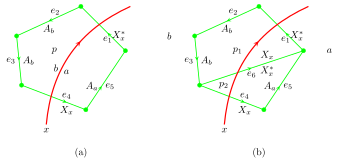
\includegraphics{figures/c13-fig14.svg}

	\caption{Example(II) of a local modification of cell decomposition used in \leref{l:invariance-under-local-moves}}
	\label{f:example2-local-modification}
\end{figure}


The contribution to projector $P$ coming from the new edge $e_6$ is:
\begin{align*}
	P_{e_6}: \kk &\rightarrow X_x \otimes X_x^*\\
	1 &\mapsto  \sum_j u_j \otimes u_j^*\\
\end{align*}

The total contribution of cells $p_1$ and $p_2$ from the right picture is
\begin{align*}
	& \sum_{j} \varphi(b_1.b_2.u_j)\ u_j^{*}(x.a)\\
	& =\sum_{j} \varphi(b_1.b_2.u_j u_j^{*}(x.a) )\\
	& =\varphi(b_1.b_2.x.a)
\end{align*}
This contribution is the same as that of the original pentagon shown in the left part of the figure. The proof for the invariance of functor $Z$ under the remaining local moves can be constructed similarly.


\section{TQFT as special case of defect TQFT}\label{s:tqft-as-dtqft}
A TQFT ( without defect ), with or without boundary, can be thought of as a special case of defect TQFT on a closed manifold. A TQFT without a boundary can be simply obtained by choosing a coloring which contains no defects.

\begin{equation}
	Z^{\mathrm{without\ defect}}_{A} (M) = Z^{\mathrm{defect}} (M; \mathrm{Coloring}={\{A\} ,M_1= \emptyset,M_0=\emptyset})
\end{equation}

We can also get a TQFT, described by separable symmetric Frobenius algebra $A$, on manifold $M$ with a boundary $\partial M$, by choosing appropriate coloring in a defect TQFT. This time, the coloring consists of a defect line $X_{\partial M}$ that runs along the boundary of $M$. This defect TQFT is defined on a closed manifold $\widetilde{M}$ that is an extension of $M$. The region of $\widetilde{M}$ lying outside $M$ is colored by the algebra $\kk$. The region $M$ is colored by algebra $A$. The defect $X_{\partial M}$ is thus an A-module, and in physics language, it separates the ``non-trivial phase'' $A$ from the ``trivial'' phase. For example, the following figure shows a defect TQFT equivalent to a TQFT with a boundary.


\newcommand{\picone}{%
	\vcenter{\hbox{%
			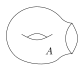
\includegraphics{figures/c13-fig15.svg}%
	}}%
}

\newcommand{\pictwo}{%
	\vcenter{\hbox{%
			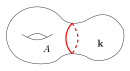
\includegraphics{figures/c13-fig16.svg}%
	}}%
}

\begin{equation}
\picone=U\left(\pictwo\right),
\end{equation}
where $U$ is a forgetful functor that erases the phase labelled by $\kk$, and removes all defect lines. See \cite{carqueville} for detailed construction of a TQFT ( with or without boundary ) from a defect TQFT.

\end{defectfiguresetup}
\clearpage